\iffalse \bibliography{include/backmatter/magnus,include/backmatter/philip} \fi
\chapter{Self-Driving Truck}\label{section:data-validation}

This section introduces the result of executing parts of the experiment on a self-driving Volvo truck, depicted in figure~\ref{truck}, that participated in the Grand Cooperative Driving Challenge (GCDC) 2016 in the Netherlands. The experiment conducted on the use-case is carried out with the intention to further understand how the scheduling precision of the CPS application is impacted by the deployment context in a system with an operational full-scale vehicular CPS running simultaneously. The use-case experiment will be run on a system with a real-time enabled kernel, as the outcome from the controlled experiment has shown that an execution environment utilising a Vanilla kernel carries undesirable overhead.\\

\begin{figure}[ht]
\centering
\caption{Chalmers Revere GCDC Truck}
\label{truck}
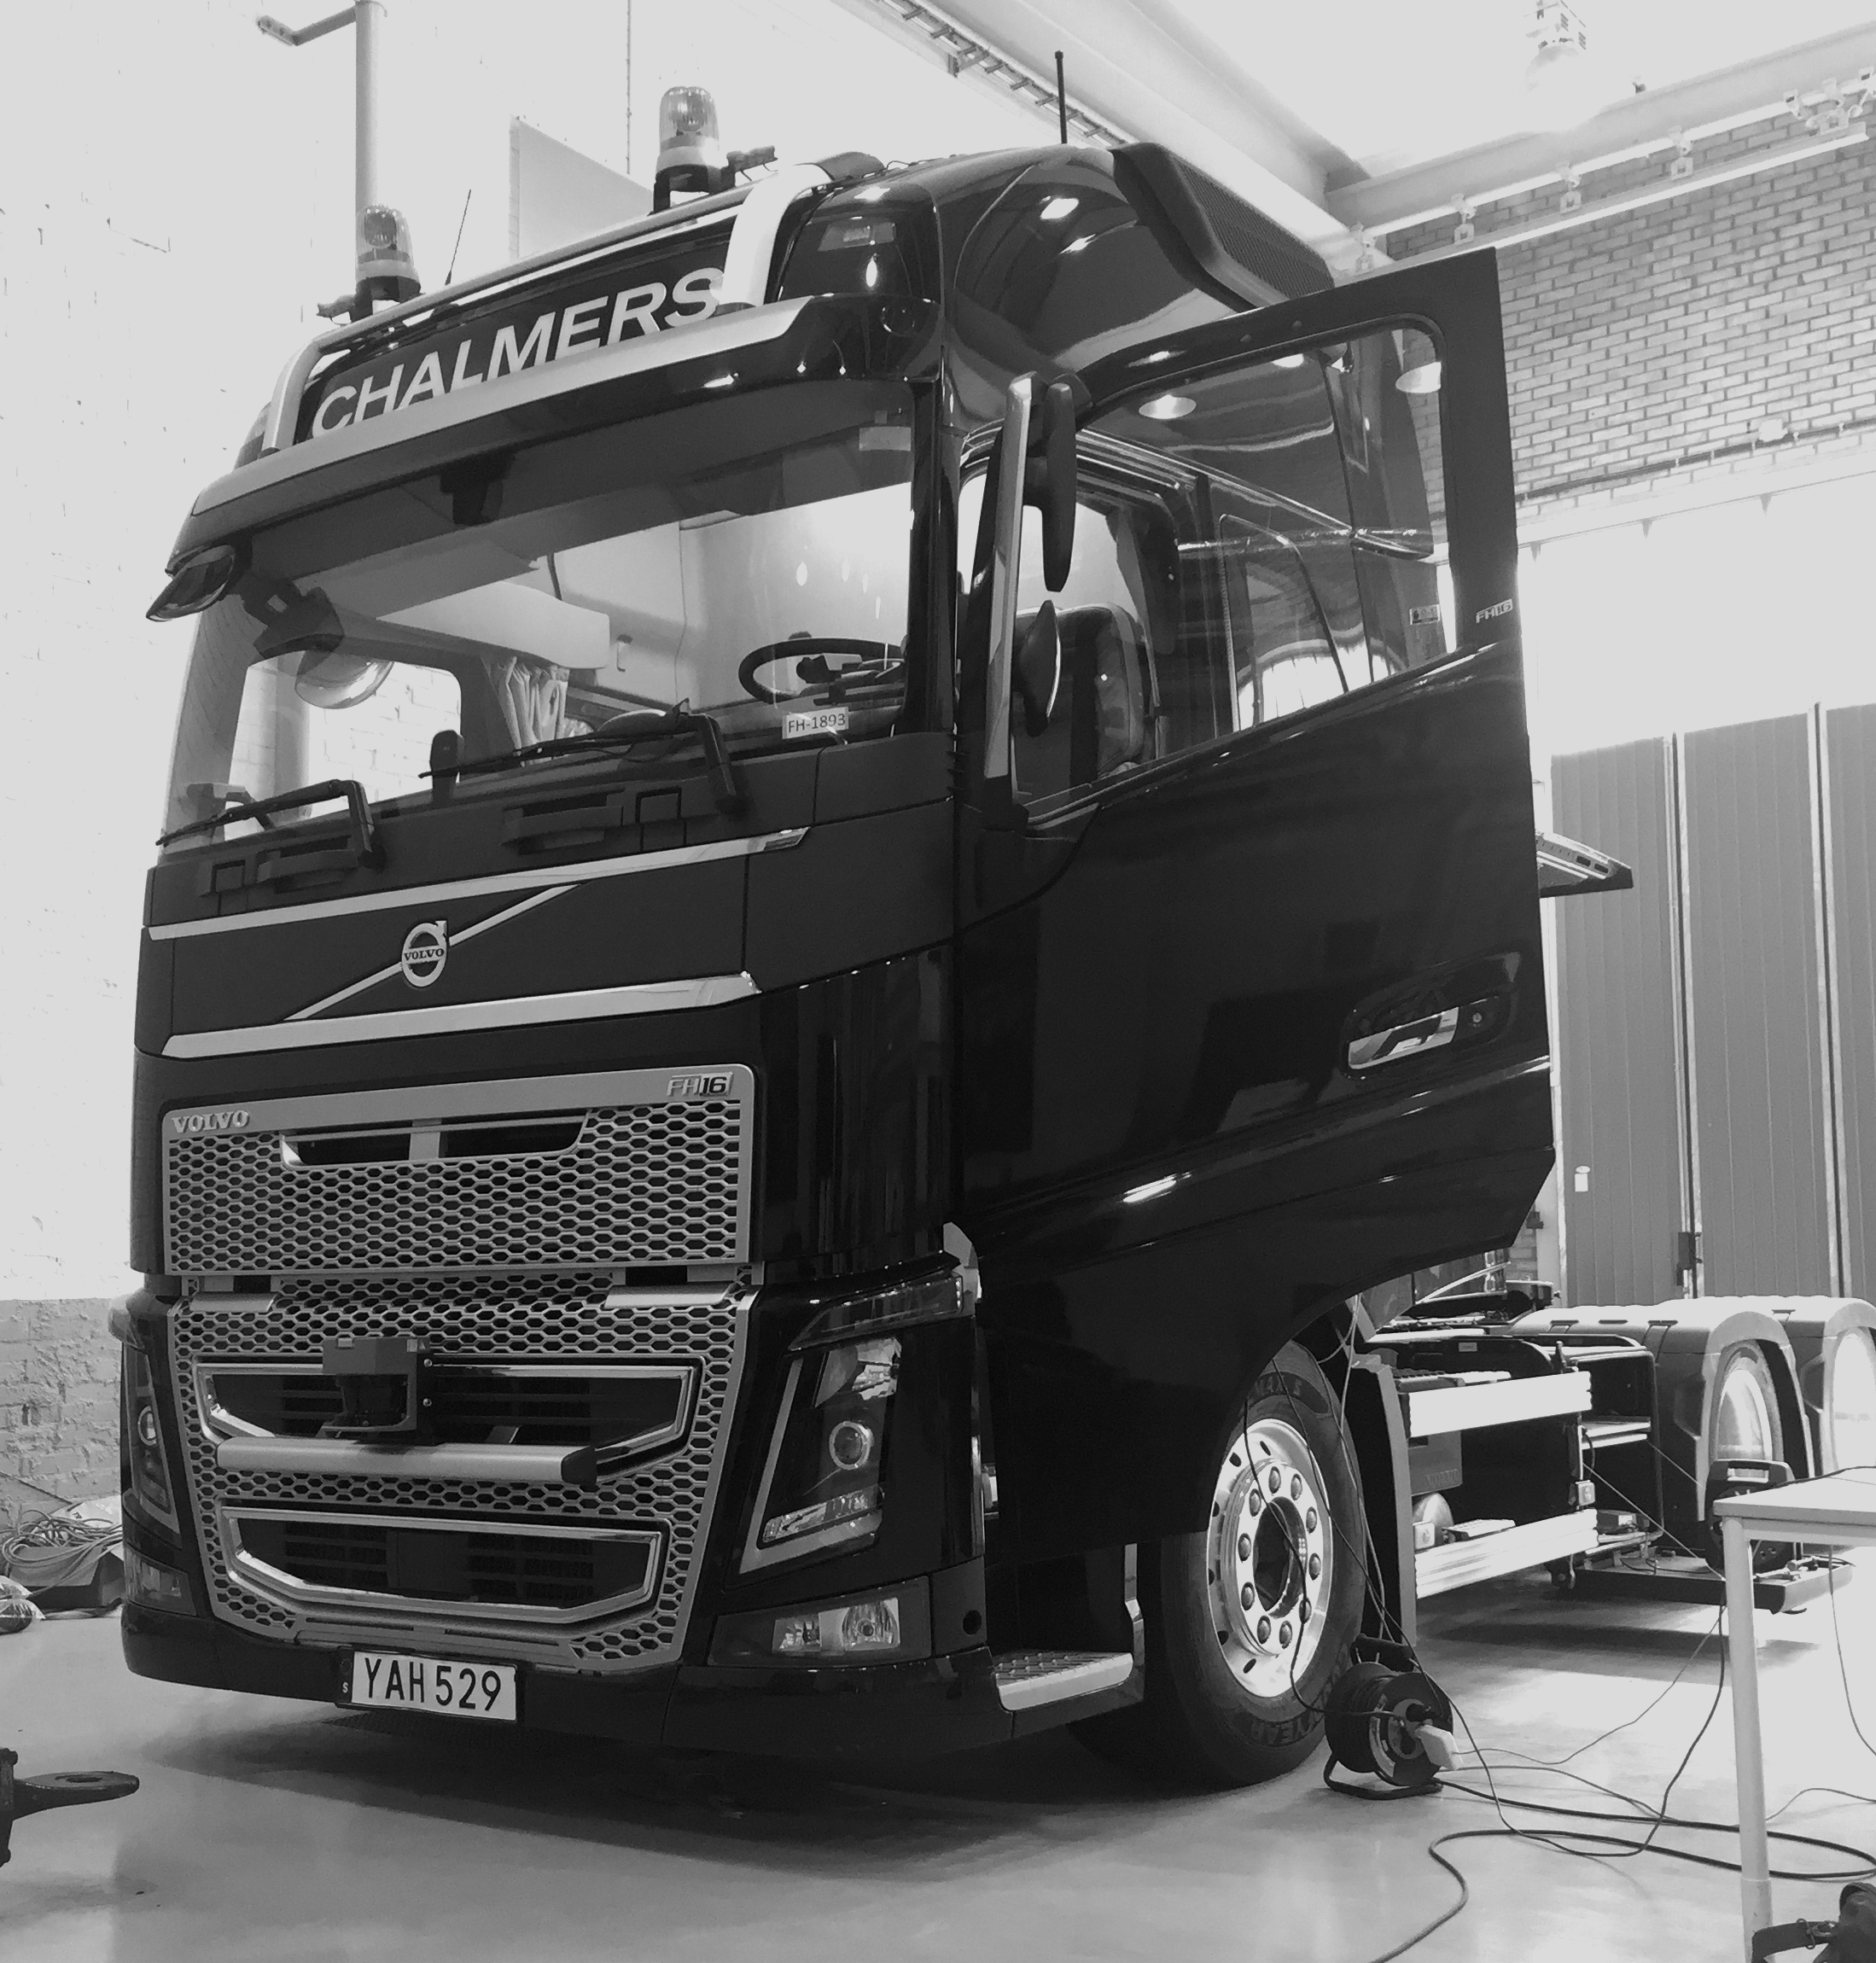
\includegraphics[width=0.4\textwidth]{./figure/truck.png}
\end{figure}


\section{Method}
\label{sec:truck-method}

This section is aimed at providing the method of the experiment conducted on the uncontrolled environment of the use-case scenario.


\subsection{Experimental Units}
\label{sec:truck-expun}

A decision to exclusively run the Pi Component is made as the self-driving truck implements a networked camera setup and hence does not have the same camera implementation as the controlled target system (section~\ref{section:hw-env}). The Pi Component presented in section~\ref{section:exp-units} is executed on a target system identical to the one used during the controlled experiments. The computer is connected to hardware components mounted to a Volvo FH16 truck. As the use-case data is extracted using the Pi Component no measurements are done to understand the camera input and disk output performance for the use-case due to the priority of building an understanding of how the scheduling precision behaves with the runtime load of the self-driving truck.\\

To understand how Docker impacts the scheduling precision on the use-case, the experimental unit is executed first natively and secondly within a Dockerized container. The runtime properties of Docker are presented in table \ref{docker-parameters-truck}. Docker version 1.11.1 is used for the analysis procedure and the Docker daemon is set to use the \texttt{overlayfs} storage driver.



\begin{table}[ht]
\centering
\caption{Docker Image Runtime Properties}
\label{docker-parameters-truck}
\begin{tabular}{|l|p{10cm}|}
\hline
\textbf{Parameter}           & \textbf{Description}                                            \\ \hline
\texttt{-d}                  & Run the container in detached mode.                             \\ \hline
\texttt{--net=host}          & The networking configuration is derived from the host.          \\ \hline
\texttt{--cap-add=sys\_nice} & Allow access to devices such as the web camera and the serial port. \\ \hline
\texttt{-v}                  & Mount shared filesystems from the host into the container.    \\ \hline
\texttt{-w}                  & The working directory to execute the experimental units.               \\ \hline
\end{tabular}
\end{table}


\subsection{System Load}
\label{sec:truck-load}

The major difference in comparison to the controlled experiment is that all software components required for the Volvo truck to operate in a driver-less manner is started and run in the background: this bring a more realistic operational load and consequently a less controlled environment in respect to the controlled experiment. Fifteen components are executed natively and within a Dockerized environment on the target system. These components are tasked with various responsibilities spanning from capturing satellite positioning data, reading data from the vehicle (e.g steering position), vehicle to vehicle communication and a number of camera operating components. Measurement points are captured via serial communication to measure the impact in a real use case.\\

\subsection{Target System}
\label{sec:truck-target}

Table \ref{table:hardware-truck} presents the hardware setup for the target machine upon which the experimental unit (section \ref{sec:truck-expun}) is executed. The target system is running ArchLinux operating system with a real-time enabled kernel (RT\_preempt), version 4.5.0-1. The decision to operate the system using ArchLinux is made by the REVERE development team due to their preferences and is not a variable which this research can control. However, to ensure that the execution environment is in line with the outcome from the controlled experiment, an RT\_preempt kernel is implemented.

\begin{table}[H]
\centering
\caption{Target System Hardware Specification}
\label{table:hardware-truck}
\begin{tabular}{|l|l|}
\hline
\textbf{Component} & \textbf{Specification}           \\ \hline
Processor          & Intel Core i7 3517UE 1.7 GHz     \\ \hline
Memory             & 4GB DDR3 1333/1600 SODIMM        \\ \hline
Storage Device     & 2.5" SATA HDD x 1                \\ \hline
Serial Interfaces  & \begin{tabular}[c]{@{}l@{}}USB type A x 2 for USB 2.0\\ USB type A x 2 for USB 3.0\\ DB-9 x 2 for RS-232/422/485 x 2\\ DB-9 x 4 for RS-232 x 4 \\ Isolated DB-9 x 2 for RS-232/422/485 x 2
\end{tabular} \\ \hline
\end{tabular}
\end{table}


\subsection{Variables}

The uncontrolled experiment is intended to understand the deployment context's impact on the scheduling precision. In comparison to the controlled environment the kernel is statically set to an RT\_preempt kernel and thus not used as a treatment to the use-case experiment. The deployment context is a categorical variable which holds two values, namely 1) Native and 2) Docker. Where the former is the execution of the experimental unit on the host OS and the second is the execution of the experimental unit in a Dockerized container. As the use-case scenario is a replication of the controlled environment, the same dependent variables are used for measuring the scheduling precision of the experimental unit, namely: 1) Overhead \#1, 2) Pi Algorithm, 3) Overhead \#2, and 4) Sleep. Figure \ref{pi_measure} presents the measurement points from where within the time-slice each of the dependent variables are extracted.\\


\subsection{Procedure}

The procedure is to execute the experimental unit in 2 different scenarios. The two scenarios is an alternation between two deployment contexts, namely 1) Executing natively on the host OS, and 2) Executing within a Dockerized environment. Each scenario is manually executed for $1h$ on the target machine with the Raspberry Pi SoC \cite{raspberry} hardware connected through a serial to USB device used for capturing measurement data via RS-232 serial communication.\\


\subsection{Analysis Procedure}

Analysing the data is made with a partly replicated analysis procedure used for understanding the scheduling precision of the controlled experiment. The purpose of running the uncontrolled experiment is to provide an insight to how the experimental unit's scheduling precision behave in an environment with realistic load. Each of the measurement points presented in figure \ref{pi_measure} are extracted and processed by calculating the duration between the points using a script. The durations is then analysed by building bar charts to illustrate the scheduling precision which is intended to provide an overview of all data points extracted. Furthermore, a table of sample size, means, and standard deviations is constructed to provide the descriptive statistics of the generated bar charts. Lastly, a one-way multivariate analysis (MANOVA) is conducted to understand how the deployment context impact the scheduling precision and an effect size ($\eta^{2}$) between the deployment context and scheduling precision is calculated to bring a more detailed understanding of what impact the deployment context has on the scheduling precision.\\



\section{Results}
\label{section:results-usecase-experiment}

This section presents the results extracted from the experiment conducted on the use-case of the self-driving truck in the Chalmers Revere Lab. The goal is to understand and provide an insight in how the deployment context impacts the experimental units within an environment which have realistic system load.\\


\subsection{Descriptive Statistics}

\begin{table}[ht]
\centering
\caption{Descriptive Statistics}
\label{tab:desc-table-pi-truck}
\renewcommand{\arraystretch}{1.2}
\begin{tabu}{L{2.4cm}lcccl}
\parbox{2.4cm}{\centering \textbf{Type of variable}}                       & \textbf{Variable}     & \textbf{N}    & \textbf{Mean} & \parbox{1.8cm}{\centering \textbf{Std.dev. ($ns$)}}  & \parbox{1.5cm}{\centering \textbf{Scale}} \\ \tabucline[2pt]{-}
\multirow{3}{*}[-.1em]{\parbox{2.8cm}{\centering Independent variables}}  & Deployment Context & 719 996 & N/A  & N/A & Nominal  \\ \hline
\multirow{4}{*}[-.2em]{\parbox{2.8cm}{\centering Dependent variables}}    & Overhead \#1  & 719 996 & 29 268 & 8 506 & Ratio     \\
                                      & Pi Algorithm          & 719 996   & 8 018 460   & 5 452 & Ratio     \\
                                      & Overhead \#2          & 719 996   & 54 993      & 26 340    & Ratio     \\
                                      & Sleep                 & 719 996   & 1 897 278   & 31 649 & Ratio     \\ \hline
\end{tabu}
\end{table}

The results shown in figure \ref{fig:truck-std-chart-noload} show that there exists a difference between the two deployment contexts in the load environment introduced by the other components running on the same system. The difference indicates that the deployment context has an impact on how deterministic a system is as native fluctuates roughly $40\%$ less than the Docker deployment context. Running a statistical test to understand the cause and effect relationship between the deployment context and the dependent variables resulted in a $\eta^{2}=0.504$ which relates to a medium effect size between deployment context and the dependent variables according to Cohen's D ($\eta^{2} > 0.5$). Figure \ref{fig:truck-mean-chart-noload} show that there exists no violations for the average time deadline for either of the two execution environments.\\


\pgfplotstableread[col sep = semicolon]{data/truck/colsd_load.csv}\mydatanoload
\begin{figure}[ht]
\caption{Standard deviation of execution environments with real-life load \textit{(lower is better)}}
\label{fig:truck-std-chart-noload}
\begin{tikzpicture}
\begin{axis}[
      xbar stacked,
      width=\textwidth*.95,
      height=\textheight*.19,
      xlabel={},
      ytick=data,
      xmin=0,
      % xmax=1.15,
      enlarge y limits={abs=1},
      y dir=reverse,
      xlabel={$ns$ std. dev.},
      yticklabels={Native [RT],Docker [RT]},ytick={1,...,2},
      point meta={x*100},
      legend style={
                draw=none, % ?
                text depth=0pt,
                at={(0.5,-0.38)},
                anchor=north,
                legend columns=-1,
                % default spacing:
                column sep=1cm,
                % the space between legend image and text:
                /tikz/every odd column/.append style={column sep=0cm},
            }
        ] %first axis

\addplot+[draw opacity=0,fill=orange,xbar,area legend] table[y=scenario,x=odv_oh1]{\mydatanoload};
\addplot+[draw opacity=0,fill=blues3,xbar,area legend] table[y=scenario,x=pi_calc]{\mydatanoload};
\addplot+[draw opacity=0,fill=blues5,xbar,area legend] table[y=scenario,x=odv_oh2]{\mydatanoload};
\addplot+[draw opacity=0,fill=blues1,xbar,area legend] table[y=scenario,x=sleep]{\mydatanoload};

\legend{\scriptsize Overhead 1,\scriptsize Pi calculation,\scriptsize Overhead 2,\scriptsize Sleep};
\end{axis}
\end{tikzpicture}
\end{figure}


\pgfplotstableread[col sep = semicolon]{data/truck/colsum_load.csv}\mydatanoload
\begin{figure}[ht]
\caption{Mean consumed of time-slice with use-case load \textit{(closer to 100\% is better)}}
\label{fig:truck-mean-chart-noload}
\begin{tikzpicture}
\begin{axis}[
        xbar stacked,
        width=\textwidth*.95,
        height=\textheight*.19,
        xlabel={},
        ytick=data,
        xmin=0,
        xmax=1.15,
        y dir=reverse,
        xlabel={$\%$ of time-slice},
        enlarge y limits={abs=1},
        yticklabels={Native [RT],Docker [RT]},ytick={1,...,2},
          x label style={at={(axis description cs:0.5,-0.1)},anchor=north},
        xticklabel={\scriptsize\pgfmathparse{\tick*100}\pgfmathprintnumber{\pgfmathresult}\%},
        point meta={x*100},
        legend style={
                draw=none, % ?
                text depth=0pt,
                at={(0.5,-0.35)},
                legend cell align=left,
                anchor=north,
                legend columns=-1,
                % default spacing:
                column sep=1cm,
                % the space between legend image and text:
                /tikz/every odd column/.append style={column sep=0cm},
            }
        ] %first axis


\draw[black, dotted] (axis cs:1,-2) -- (axis cs:1,11);
\addplot+[draw opacity=0,fill=orange,xbar,area legend] table[y=scenario,x=odv_oh1]{\mydatanoload};
\addplot+[draw opacity=0,fill=blues3,xbar,area legend] table[y=scenario,x=pi_calc]{\mydatanoload};
\addplot+[draw opacity=0,fill=blues5,xbar,area legend] table[y=scenario,x=odv_oh2]{\mydatanoload};
\addplot+[draw opacity=0,fill=blues1,xbar,area legend] table[y=scenario,x=sleep]{\mydatanoload};

\legend{\scriptsize Overhead 1,\scriptsize Pi calculation,\scriptsize Overhead 2,\scriptsize Sleep};
\end{axis}
\end{tikzpicture}
\end{figure}



\subsection{Hypothesis Testing}

Table \ref{tbl:manova-pi-truck} presents the resulted MANOVA and effect size calculated from the data derived from the uncontrolled experiment.


\begin{landscape}
\begin{table}[ht]
\small
\centering
\caption{MANOVA and Effect Size}
\label{tbl:manova-pi-truck}
\renewcommand{\arraystretch}{1.2}
\begin{tabu}{r|cKKccccD}
                                & \textbf{Df} & \textbf{Pillai} & \textbf{Wilks} & \textbf{approx F} & \textbf{num Df} & \textbf{den Df} & \textbf{Pr(>F)} & \textbf{$\eta^{2}$}   \\  \tabucline[2pt]{-}
\textbf{deployment context}     & 1           & 0.50408         & 0.99996        & 182 958           & 4               & 719 993         & {< 2.2e-16}     & 0.5040774   \\
\textbf{Residuals}              & 719 996
\end{tabu}
\end{table}

\begin{table}[ht]
\centering
\caption{Coefficient between treatment and dependent variable ($ns$)}
\label{tbl:coef-pi-truck}
\renewcommand{\arraystretch}{1.2}
\begin{tabu}{r|rlrlrlrl}
\multicolumn{1}{c}{\textbf{}} & \multicolumn{2}{c}{\textbf{Overhead \#1}} & \multicolumn{2}{c}{\textbf{Pi Algorithm}} & \multicolumn{2}{c}{\textbf{Overhead \#2}} & \multicolumn{2}{c}{\textbf{Sleep}} \\ \tabucline[2pt]{-}
\textbf{(Intercept)} & 27 944                                     &                               & 8 017 426                                   &                               & 36 462                                     &                               & 1 918 167                            &                               \\
\textbf{deployment}  & 2 648                                      & (0,095)                         & 2 067                                      & (0,000)                         & 37 062                                     & (1,016)                         & -41 777                             & (-0,022)                       
\end{tabu}
\end{table}
\end{landscape}



















